\subsection*{1.3 Elektrischer Widerstand R [$\Omega$]}

Widerstand: \mathbox{R = \frac{U}{I}, I \sim U}

\begin{tabular}{c c}
    Ohmsche Leiter & nicht-ohmsche Leiter \\
    $I = \frac{U}{R}$ & $R_{\text{diff}} = \frac{dU}{dI}$\\
    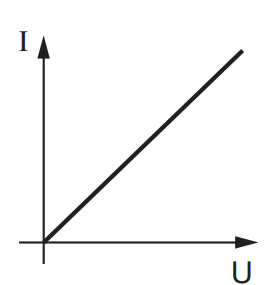
\includegraphics[width = 30mm]{src/images/plot_ohmscher_leiter.png} & 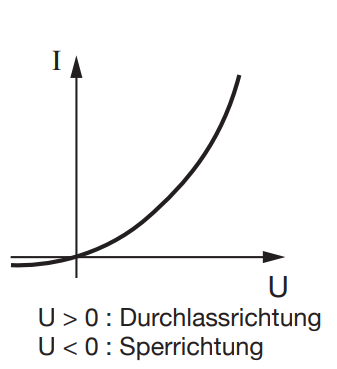
\includegraphics[width = 30mm]{src/images/plot_nicht-ohmscher_leiter.png}
\end{tabular}

\subsubsection*{Spezifischer Widerstand}
nach Grösse:

\vspace{-1mm}
\begin{minipage}{0.49\linewidth}
    \begin{footnotesize}
        \begin{center}
            \mathbox{
                R = \rho \frac{l}{A}
            }
        \end{center}
    \end{footnotesize}
\end{minipage}
\begin{minipage}{0.5\linewidth}
    \begin{scriptsize}
        \begin{center}
            \begin{align*}
                l &= \text{Leiterlänge}
                \\A &= \text{Leiterquerschnitt} 
                \\\rho &= \text{spezifischer Widerstand}
                \\  K &= \frac{1}{\rho} = \text{Spezifische Leitfähigkeit}
            \end{align*}
        \end{center}
    \end{scriptsize}
\end{minipage}
\vspace{1mm}

nach Temperatur:

\vspace{-1mm}
\begin{minipage}{0.49\linewidth}
    \begin{footnotesize}
        \begin{center}
            \mathbox{
                \rho(T) = \rho_0 (1 + \alpha(T - T_0))
            }
        \end{center}
    \end{footnotesize}
\end{minipage}
\begin{minipage}{0.5\linewidth}
    \begin{scriptsize}
        \begin{center}
            \begin{align*}
                \rho_0 &= \text{spezifischer Widerstand bei } T_0
                \\T_0 &= \text{Bezugstemperatur}
                \\\alpha &= \frac{1}{K} =\text{Temperaturkoeffizient}
            \end{align*}
        \end{center}
    \end{scriptsize}
\end{minipage}
\vspace{1mm}